\chapter{Introduction}\label{chap:intro}
Fundamental problems in machine learning (ML) require making decisions under uncertainty. Several ML applications assume the empirical data to be sampled from an unknown distribution and train a probabilistic model to match the true distribution. This naturally makes the task of comparing distributions ubiquitous in ML \citep{Frogner15,wgan17,Genevay2017LearningGM,bottou2017geometrical,Courty17domAda,damodaran2018deepjdot,cadgan,jumbot,kernelicml23,chen2023plot}. We present a brief introduction to the approach of comparing distributions centered around the concepts of optimal transport.
\section[Introduction to Optimal Transport]{Introduction to Optimal Transport}
Optimal Transport (OT) theory, originating from the seminal work of \cite{monge}, has become a fundamental tool that induces a geometric notion to compare distributions. The standard measure-theoretic arguments introduce us to the concept of transforming a probability measure into another. Given a cost function over the support of the distributions, the Monge-OT problem \citep{monge} searches for such a transformation function that incurs the least transformation cost. This formulation was relaxed by Kantorovich \citep{KatoroOT}, who posed the problem in terms of a probabilistic transport coupling, also known as the OT plan. Unlike the case of the Monge-OT problem, the solution to the Kantorovich-OT problem always exists. Further, \cite{brenier} showed conditions under which the solutions to these two problems coincide.

OT provides a valid distance metric over distributions whenever the cost function over the support of the distributions is a valid metric~\citep{villanioldnew}. The family of metrics induced by the OT formulation is popularly known as $p$-Wasserstein ($p>1$) metrics. Furthermore, the transport coupling or the OT plan obtained with the Kantorovich-OT formulation provides an optimal alignment between the support of the two distributions. These theoretical results also extend to the OT formulation over unnormalized measures \citep{Liero2018}. However, despite these appealing features, there were computational bottlenecks in employing such OT-based methods in large-scale applications. The seminal work by \cite{cuturi13a} alleviated these challenges by proposing an entropy-regularized OT formulation that enjoyed scalable solvers. This led to the adoption of OT-based methods in several applications like supervised learning \citep{Frogner15}, generative modeling \citep{wgan17,Genevay2017LearningGM,ROT}, tackling distributional shifts \citep{Courty17domAda,courty17b,damodaran2018deepjdot,jumbot}, solving alignment-based problems \citep{alvarez18wordEmb,arase-etal-2023-unbalanced}, modeling cell-population dynamics \citep{bioapp19,TNet20,Cuturi22,cellot}, and many more. We refer the readers to \cite{khamis24OT} and \cite{Torres21} for recent surveys on this. A detailed review of different variants of the OT formulation and their computational aspects can be found in \cite{peyre2019computational}.

The feature of inducing a distance between distributions by leveraging the geometry over their support is particularly beneficial in applications when the distributional supports exhibit non-Euclidean geometry, like distributions over graphs \citep{GOT} or over more structured entities like datasets \citep{alvarezmelis2020geometricdatasetdistancesoptimal}. Another key aspect of OT distances is their applicability when the supports of the two distributions do not overlap. An example is demonstrated in Fig~\ref{fig:weak-conv} where the convergence of the Dirac measures is mimicked in the corresponding OT distances but is not reflected in the distances/divergences obtained with KL-divergence or Total Variation (TV) distances (two of the popular divergence functions).


\begin{figure}[t]
    \centering
    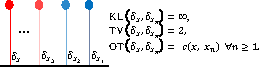
\includegraphics[width=0.5\linewidth]{intro-chapter/weak-conv2.pdf}
    \caption[Illustrating the geometry-induced OT distance and comparing with other divergences as a Dirac measure converges (in law) to another.]{Comparing KL-divergence, Total Variance (TV) distance and the $p$-Wasserstein distance (OT distance) as a Dirac measure converges (in law) to another. The geometry over the support points is captured by the OT distance as it lifts the ground metric, $c$, to provide a metric over the measures.}\label{fig:weak-conv}
\end{figure}
Despite these attractive properties, a notable drawback of the Wasserstein metrics is the need for exponential no. of empirical samples to estimate the true distances in high dimensions \citep{dudley1969,nilesweed2019estimation,Chewi2024StatisticalOT}. Recent approaches to alleviate this issue have employed the Sliced-Wasserstein formulation, which involves averaging the Wasserstein distances obtained with several one-dimensional projections of the measures \citep{bonet2023leveraging}. This approach has its own set of computational challenges \citep{peyre2019computational}. Our work, on the other hand, is focused on devising careful choices of kernel-based regularization with sample-efficient estimation guarantees that are also computationally efficient.

\section{Motivation for the Thesis}\label{motive}
In our preceding discussions, we highlighted that the statistical estimation of the Wasserstein metric in higher dimensions is known to be cursed with dimensionality. This estimation problem is known to be as challenging as the problem of estimating the involved densities themselves \citep{nilesweed2019estimation}. On the other hand, the Kernel Mean Embeddings of the corresponding densities can be estimated with sample complexity that is independent of the dimension \citep{Muandet_2017}. Additionally, it is established that with Characteristic kernels (e.g., Kronecker Delta kernel over the discrete domain, RBF kernel over the continuous domain), an injective mapping exists between densities and their Kernel Mean Embeddings \citep{Muandet_2017}. This motivated our exploration to study the effect of kernel-based regularization in OT formulations.

Although kernel methods have been widely used in several ML applications~\citep{Hofmann_2008, gretton12a,Li17,Li21,nguyen20, kernelaistats22, kernelicml23, kernelicml24}, the study of statistical and empirical properties of kernel-methods in OT gained little to no attention in the prior works. \cite{zhangotkernel19} presented a reformulation of Kantorovich-OT in the RKHS space, but their focus was on the computational aspects of the formulation under the specific assumptions of the pushforward measures on RKHS being Gaussians. \cite{ot-kme} posed the problem of statistical OT as that of learning the corresponding Kernel Mean Embeddings of the transport plan and proved dimension-free estimation rates. However, several questions, like the metric properties of the resulting divergence, the scope of extending the formulation to unnormalized measures, the applicability to OT between conditionals, and the questions on scalability to large-scale ML applications, are left unanswered in \cite{ot-kme}.

This leads us to pose the first set of questions on statistical and computational aspects of the OT formulation with kernel-based regularization.
\begin{definitionBoxIntro}
\begin{enumerate}[labelwidth=1em, leftmargin=1em, align=left]
    \item[\textbf{(I.I)}] Would kernel-based regularization for OT also lead to novel metrics over measures, analogous to the ones studied with the regularization based on KL divergence~\citep{Liero2018} or the TV distance~\citep{Piccoli2014GeneralizedWD}?
    \item[\textbf{(I.II)}] Would the statistical complexity of the resulting OT divergence/metric be like the dimension-free sample complexity of MMD, or would these stay cursed with dimensionality like with the Wasserstein?
    \item[\textbf{(I.III)}] Would the resulting formulation exhibit computational efficiency like the popular entropy-regularized OT divergence solved with the Sinkhorn algorithm?
\end{enumerate}
\end{definitionBoxIntro}
The discussion on the computational efficiency with entropy-regularized OT variants leads us to our next research problem. A notable drawback of the popular Sinkhorn algorithm, employed to solve the entropy-regularized OT, is that it results in an OT plan with each entry being strictly positive. Such dense entropic-OT plans often hinder the interpretability of alignments obtained \citep{swanson-etal-2020-rationalizing}. While at first, it may seem that the issue of non-sparsity could be alleviated by lowering the coefficient of entropic regularization ($\epsilon$), this results in the Sinkhorn algorithm becoming numerically unstable \citep[Remark (4.7)]{peyre2019computational} due to the algorithmic steps involving the factor of $(1/\epsilon)$. We make a critical observation that the smoothness induced by kernel-based regularizers like the squared-MMD can replace the entropic regularization and enable efficient learning of the desired solution structure.

With these observations, we present our second set of research questions for the problem of OT with sparsity constraints.
\begin{definitionBoxIntro}
\begin{enumerate}[labelwidth=1em, leftmargin=1em, align=left]
\item[\textbf{(II.I)}] Can the smoothness in OT objective resulting from squared-MMD regularization help design a scalable framework to replace the dense entropic-OT-plan with a solution that exhibits controlled sparsity?
\item[\textbf{(II.II)}] Can we further achieve controlled structured sparsity in the OT plan, which would directly aid the applications demanding budget-constrained mappings?
\end{enumerate}
\end{definitionBoxIntro}
Deferring the discussion on our contributions to these open questions, we first present the next challenging setup, which we propose to tackle with kernel-based regularization in OT. The setup involves solving an OT problem between conditional measures when empirical samples are available from joint distributions rather than their corresponding conditionals. The need to compare conditional distributions frequently arises in ML, for example, in the supervised training of discriminative models or while learning conditional generative models. As the input covariates in such applications are (typically) continuous, the samples are observed from the joint distribution of covariates corresponding to the input and the label. It is well known that estimating conditionals is a significantly more challenging problem than estimating joints \citep[Sec. 2]{LiNeykovBalakrishnan}. Further, when the distributions of input covariates in the two joints are not the same, merely comparing the joints is not equivalent to comparing the corresponding conditionals. Such a setup demands a new formulation for solving an OT problem between conditionals.

Motivated by the sample-efficient estimation of Kernel Mean Embeddings of conditionals from the given joint samples \citep{gretton}, we pose our third set of research questions in the discussed context of formulating an OT problem over conditionals.
\begin{definitionBoxIntro}
    \begin{enumerate}[labelwidth=1em, leftmargin=1em, align=left]
    \item[\textbf{(III.I)}] Can we formulate a statistically consistent OT problem between empirical conditional measures when the samples are provided from the joints alone?
    \item[\textbf{(III.II)}] Can the corresponding conditional-OT-plan-based estimators be modeled efficiently to act as conditional generators?
    \end{enumerate}
\end{definitionBoxIntro}

\textit{\textbf{By providing affirmative answers to these challenging questions,
this thesis endeavors to provide a rigorous theory for our novel OT formulations with kernel-based regularizations that exhibit appealing statistical and computational properties. The central thesis of this work is that kernel-based MMD regularization in OT enables us to solve all the three sets of challenges discussed above.}}

\section{Contributions of the Thesis}
We begin by answering the first set of research questions through our theoretical and empirical study of kernel-regularization in OT (Chapter~\ref{chap:ch1}), whose contributions are summarized below.

We study the MMD-regularized OT formulation that softly matches the transport plan’s marginals with the given source and target measures using kernel-based MMD regularizers.
Our first technical contribution includes deriving and analyzing the dual of the MMD-regularized OT problem and proving that it induces novel metrics. We further show that this metric exhibits statistical efficiency like the MMD with a sample complexity of $O(m^{-1/2})$, where $m$ is the number of samples, which is independent of dimensions. We present finite-dimensional convex-program-based estimators for this problem and the corresponding barycenter problems. With certain assumptions, we also prove that the estimation error with this finite parameterization also comes out to be $O(m^{-1/2})$. To the best of our knowledge, such estimation bounds with finite parameterization of the OT plan are not known for other variants of OT. Our formulation and proofs extend to the case of unnormalized measures and not just probability distributions. It is also noteworthy that most of the theoretical proofs we present extend to the case when a general Integral Probability Metric (IPM), not necessarily kernel-based MMD, is used for the regularization of the marginals. Moreover, with a regularization based on squared-MMD, we leverage the smoothness of the resulting optimization objective and propose scalable solvers for the problem that can efficiently handle large datasets. Empirically, we show improvements over applications like domain adaptation, two-sample hypothesis testing, few-shot classification, and more.

Our next work (Chapter~\ref{chap:ch2}) answers the second set of research questions raised in the previous section. Our contributions from this work are summarized below.

We leverage the proposed kernel-regularized OT formulation from the preceding discussion to induce structured sparsity in the transport plans. The entropy-regularized OT variants, while computationally efficient, result in dense (and less interpretable) transport plans where each entry is strictly positive. By showing the equivalence between the OT problem with squared-MMD-based regularization and a submodular maximization problem, we propose a framework to efficiently induce sparsity in OT plans. We highlight that such an equivalence may be of independent interest beyond inducing sparsity in the transport plan. Our framework also allows for incorporating structural patterns in the OT plan, such as column-wise sparsity or row-wise sparsity. We improvise the existing algorithms to provide more efficient approximation algorithms for solving the resulting submodular maximization problem. Our approach not only showcases a better optimization quality but also improves downstream ML applications like that of designing network topology, aligning words in sentence pairs and learning sparse-mixture-of-expert models.

We answer the third set of questions raised in the preceding section through the following contributions (Chapter~\ref{chap:ch3}).

A significant contribution of this thesis is formulating a statistically consistent OT problem over empirical conditional measures, with an estimation error of $O(m^{-1/4})$, where $m$ is the number of samples. These problems are particularly challenging when the conditioned variable is continuous, where we typically do not have access to samples corresponding to the values of the conditioned variables, but rather, the samples provided are from joint distributions. Our approach uses kernelized least-squares-based MMD regularizers to implicitly match the transport plan’s marginals with the empirical conditionals, providing a consistent OT formulation for comparing conditional measures. The property of the MMD metric that allows comparing measures with non-overlapping support helps us to model the conditional transport plan through implicit models, with which we also showcase the statistical consistency guarantees. We empirically verify the correctness of the proposed estimator and evaluate its utility on downstream applications, such as conditional generation for modeling cell population dynamics and prompt learning for few-shot classification.

These contributions, expanded in the forthcoming chapters, corroborate the thesis idea of improving OT formulation using kernel methods.
\section{Organization of the Thesis}
The organization of this thesis is detailed as follows.\newline\newline
\noindent\textbf{Chapter \ref{chap:intro}} presents an introduction to the problem of Optimal Transport (OT) with a focus on the Kantorovich-OT variant, which is central to our work. We discuss various applications of the OT-based distance function and the corresponding transport plan. We then shed some light on the open problems in OT and motivate our contributions. More specifically, we pose three sets of research questions and then summarize our contributions to improving the OT formulation using kernel-based regularization to answer these.
\newline
\newline
\noindent\textbf{Chapter \ref{chap:chbg}} provides the mathematical background relevant to the core concepts used in the thesis. This chapter is broadly divided into two parts. In the first part, we focus on the mathematical background for OT, and in the second part, we discuss the relevant mathematical background for kernel-related concepts. 

We begin with the OT formulation given by Kantorovich and discuss its variants. We then familiarize the reader with relevant statistical and computational results in estimating the OT distance when finitely many samples are provided.

In the second part, we begin the discussion on kernels by introducing the notion of kernel functions. We then present the kernel-based MMD metric, a core concept used in all the subsequent chapters. We discuss the statistical efficiency of the MMD metric and highlight the ease of computing MMD when finitely many samples are provided.
\newline
\newline
\noindent\textbf{Chapter \ref{chap:ch1}} presents our first contribution as a theoretical and empirical study of the proposed OT formulation with kernel-based regularization. This chapter is based on our published journal, \cite{mmd-uot}, and answers the first set of questions that motivated our research (Sec.~\ref{motive}).
\newline
\newline
\noindent\textbf{Chapter \ref{chap:ch2}} discusses our proposed framework for inducing structured sparsity in the OT plan using the kernel-regularized OT formulation. This chapter is based on our published work, \cite{sot}, and answers the second set of questions that motivated our research (Sec.~\ref{motive}).
\newline
\newline
\noindent\textbf{Chapter \ref{chap:ch3}} presents our novel statistically consistent OT formulation over conditional measures leveraging the kernel-regularized OT formulation. This chapter is based on our published work, \cite{cot}, and answers the third set of questions that motivated our research (Sec.~\ref{motive}).
\newline
\newline
\noindent\textbf{Chapter \ref{chap:conclude}} concludes the thesis and lists open problems that arose from our research. We also discuss potential directions for future work on improving the OT formulation as well as for the study of the interplay between OT and kernel methods.
\newline
\newline
\noindent\textbf{Appendices \ref{APP:A}}, \textbf{\ref{APP:B}} and \textbf{\ref{APP:C}} provide additional theoretical and experimental details for Chapters \ref{chap:ch1}, \ref{chap:ch2} and \ref{chap:ch3}, respectively. These main chapters present the statements of our theoretical results, with the proofs deferred to the corresponding appendices.